\section{OT-Security}

\subsection{Abgrenzung IT-Security und OT-Security}

Die Unterscheidung zwischen IT-Security und OT-Security ist in der Sicherheitsarchitektur industrieller Systeme von zentraler Bedeutung. Während IT-Security hauptsächlich darauf abzielt, Informations- und Kommunikationstechnologien zu sichern, konzentriert sich OT-Security auf die Absicherung von Steuerungs- und Automatisierungstechnologien. Mit \ac{ot} meint es "[...] Hard- und Software, die physische Geräte, Prozesse und Ereignisse in der Institution überwacht und steuert" (\cite {ICS}, S. 9). Diese Unterschiede zeigen sich auch in der grundlegenden Denkweise: Während die \ac{it} virtuell ist, ist die OT physisch. Ein weiterer wesentlicher Unterschied liegt in den Schutzzielen, die unterschiedlich priorisiert werden. Gemäß des BSI sind die primären Schutzziele wie folgt definiert (vgl. \cite{BSI}): 
\begin{itemize}
\item \textbf{Vertraulichkeit}: Nur autorisierte Personen haben Zugriff zu den Informationen.
\item \textbf{Integrität}: Die Information wurde auf dem Transportweg nicht verändert.
\item \textbf{Verfügbarkeit}: Kommunikationsdienste stehen zu den gewünschten Zeitpunkten zur Verfügung.
\end{itemize}
Zusätzlich zu diesen Zielen spielt in der OT-Security auch das Schutzziel Safety eine bedeutende Rolle. Safety zielt darauf ab, Personen und die Umwelt vor physischen Schäden zu schützen, indem Maßnahmen ergriffen werden, um Unfälle zu verhindern oder ihre Auswirkungen zu minimieren (vgl. \cite{Safety}). Die unterschiedliche Hierarchie der Schutzziele wird in den folgenden Abbildungen veranschaulicht:
\begin{figure}[h]
    \centering
    \begin{minipage}{0.45\textwidth}
        \centering
        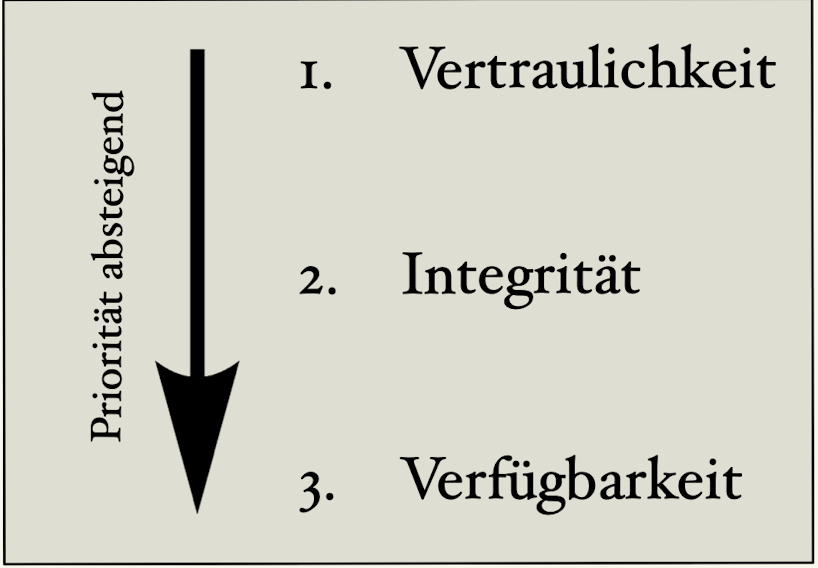
\includegraphics[scale=.4]{images/ITS.png}
        \caption{Schutzziele IT-Security}
        \label{fig:meine-grafik1}
    \end{minipage}
    \hfill
    \begin{minipage}{0.45\textwidth}
        \centering
        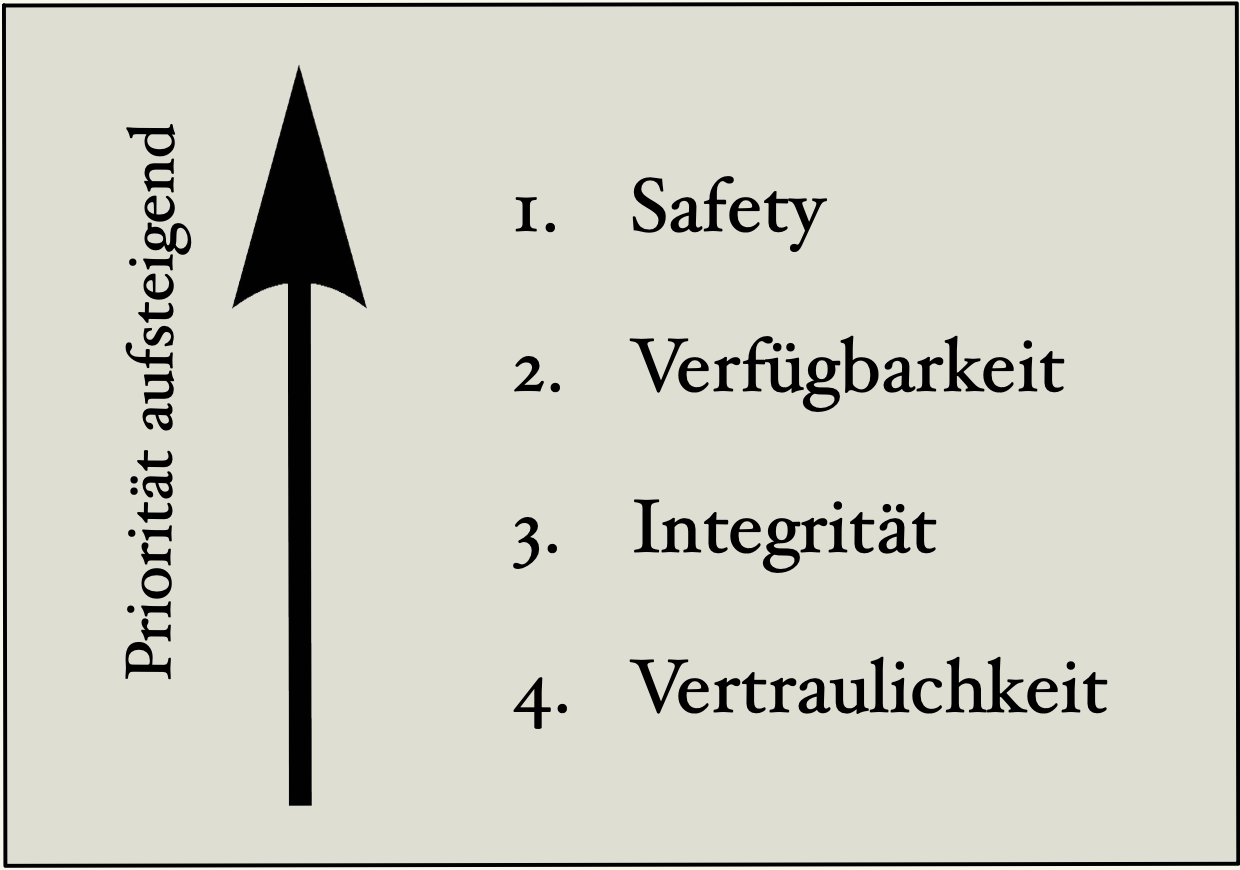
\includegraphics[scale=.37]{images/OTS.png}
        \caption{Schutzziele OT-Security}
        \label{fig:meine-grafik2}
    \end{minipage}
\end{figure}
\\ Konzeptionell verfolgen beide Ansätze verschiedene Rangordnungen der Schutzziele. Für die OT-Security ist die Verfügbarkeit industrieller Anlagen zu jedem Zeitpunkt von besonderer Bedeutung. Für Industriebetriebe ist dies essenziell, da ungeplante Ausfallzeiten enorme Kosten verursachen können (vgl. \cite{OTS/ITS}). 
\subsection{Herausforderungen}

Das ICS-Security Kompendium des \ac{bsi} ist ein Grundlagenwerk, das Organisationen dabei unterstützt, Cybersicherheitsrisiken in der OT zu erkennen und zu bewältigen, indem es Basiswissen vermittelt, Maßnahmen und Prozesse beschreibt sowie Verbindungen zu relevanten Standards und Gesetzen herstellt. Hierbei werden drei grundsätzliche Schwachstellen im OT-Umfeld definiert. Man unterteilt in Organisatorische Schwachstellen, Technische Schwachstellen und die Schwachstelle Lieferkette. 

\subsubsection{Organisatorische Schwachstellen}

Die Sicherheit industrieller Steuerungssysteme ist essenziell für die Aufrechterhaltung \ac{kritis}, aber oft durch diverse organisatorische Schwachstellen gefährdet. Eine zentrale Schwäche liegt in unzureichenden oder fehlenden organisatorischen Regelungen sowie einer mangelhaften Dokumentation zur Cybersicherheit. Diese bilden die Grundlage für effektive Entscheidungsfindung und Maßnahmen, und ihr Fehlen kann potenzielle Sicherheitslücken verursachen, die ausgenutzt werden könnten.
Ein weiteres kritisches Problem ist das unzureichende Risikomanagement in OT-Umgebungen. Ohne eine gründliche Identifikation und Bewertung potenzieller Gefahren können Schwachstellen und Bedrohungen übersehen oder falsch priorisiert werden, was zu ungeeigneten oder unzureichenden Schutzmaßnahmen führt. Dies wiederum könnte die Reaktionsfähigkeit auf Sicherheitsvorfälle beeinträchtigen und die Auswirkungen solcher Zwischenfälle verschlimmern. Ein bedeutender Aspekt ist auch die mangelnde Kommunikation innerhalb der Organisationen. Klar definierte Richtlinien und Verfahren müssen nicht nur vorhanden sein, sondern auch effektiv kommuniziert werden, um Missverständnisse zu vermeiden und sicherzustellen, dass Sicherheitsmaßnahmen korrekt umgesetzt werden. Eine unzureichende Dokumentation und Kommunikation können im Ernstfall zu erheblichen Verzögerungen bei der Fehlerdiagnose und -behebung führen, was die Ausfallzeiten und die Wiederherstellungszeiten erhöht. Ein weiteres Problem ergibt sich aus der Übertragung ungeeigneter IT-Praktiken auf das OT-Umfeld. Da IT- und OT-Systeme unterschiedliche Anforderungen und Betriebsabläufe haben, können Sicherheitsmaßnahmen und -standards aus der IT nicht einfach auf OT-Systeme übertragen werden. Dies kann zu inkonsistenten oder unzureichenden Sicherheitslösungen führen, die die spezifischen Risiken und Bedrohungen in OT-Umgebungen nicht angemessen berücksichtigen (vgl. \cite{ICS}, S. 31-34).
\clearpage
\subsubsection{Technische Schwachstellen}

In der Analyse der technischen Schwachstellen von OT-Systemen zeigt sich eine Vielzahl von Risiken, die durch unzureichende Sicherheitsmaßnahmen und veraltete Konfigurationen entstehen können. Ein zentraler Aspekt ist die unvollständige Absicherung von Fernzugängen, die autorisierten Personen ermöglichen, aus der Ferne auf Systeme zuzugreifen. Besonders relevant ist dies im Kontext zunehmender Nutzung von Homeoffice und mobilen Zugängen, jedoch sind diese Zugänge oft schlecht geschützt und können Angriffspunkte für Cyberkriminelle darstellen. Ein weiteres bedeutendes Risiko ergibt sich aus der fehlenden Überwachung der Infrastruktur, die dazu führen kann, dass sicherheitsrelevante Ereignisse und Schwachstellen nicht rechtzeitig erkannt werden. Dies birgt die Gefahr von Produktionsausfällen und Sicherheitsvorfällen, die erhebliche wirtschaftliche Schäden verursachen können. Zusätzlich sind OT-Netze zunehmend von IT-Netzen abhängig, was potenzielle Sicherheitslücken durch gemeinsam genutzte Infrastruktur und Dienste schafft. Störungen oder Angriffe in IT-Netzen können sich direkt auf OT-Umgebungen auswirken und zu schwerwiegenden Konsequenzen führen, wie z.B. Produktionsausfällen oder sogar Sicherheitsrisiken für Mensch und Umwelt. Ein weiteres kritisches Thema ist die Verwendung von Legacy-Systemen, die aufgrund ihrer veralteten Sicherheitsmechanismen und der fehlenden Herstellerunterstützung besonders anfällig für Cyberangriffe sind  (z.B. Nutzung veralteter Betriebssysteme). Diese Systeme können moderne Sicherheitsbedrohungen oft nicht effektiv abwehren und stellen somit ein erhebliches Risiko für die Sicherheit von OT-Umgebungen dar (vgl. \cite{ICS}, S. 34-39). 


\subsubsection{Schwachstelle Lieferkette}

Die Lieferketten für industrielle Steuerungssysteme haben in den letzten Jahren verstärkt das Interesse von Cyberangreifern auf sich gezogen. Diese Angreifer nutzen gezielt Schwachstellen in der Lieferkette aus, um Schadsoftware oder Hintertüren in die OT-Komponenten einzuschleusen. Dadurch können sie unautorisierten Zugriff auf KRITIS wie Stromnetze, Wasserversorgung oder Verkehrssteuerungssysteme erlangen.
Ein zentraler Aspekt sind unzureichende Sicherheitsregelungen innerhalb der Lieferkette. Wenn die Verantwortlichkeiten für die Cybersicherheit nicht klar geregelt sind, entstehen Gefahrenpunkte, da niemand sich zuständig fühlt, potenzielle Schwachstellen zu identifizieren und zu beheben. Hardware-Hintertüren sind eine weitere schwerwiegende Schwachstelle. Diese ermöglichen es Herstellern oder Dritten, verdeckte Zugänge zu Systemen oder Daten einzurichten. Solche Hintertüren können durch das Hinzufügen von Schnittstellen oder speziellen Codes in die Firmware oder das BIOS der OT-Komponenten entstehen. Die Firmware, als entscheidendes Element für die Funktion der Steuergeräte, ist ebenfalls anfällig für Schwachstellen. \clearpage \noindent Diese können durch fest einprogrammierte Zugangsdaten oder fehlerhafte Entwicklungspraktiken entstehen. Modifizierte Firmware, die durch kompromittierte Updates eingespielt wird, ermöglicht es Angreifern, Geräte fernzusteuern oder sensible Daten auszulesen. Die Kryptographie, die zur Sicherung von Daten verwendet wird, ist nicht immun gegen Schwachstellen. Fehlerhafte Implementierungen oder veraltete Verfahren können es Angreifern erleichtern, verschlüsselte Daten zu entschlüsseln oder Manipulationen vorzunehmen. Neben der Firmware sind auch Anwendungssoftware und deren Integration in die IT-Infrastruktur potenzielle Einfallstore für Angreifer. Standard IT-Betriebssysteme wie Windows, die für diese Anwendungen genutzt werden, sind selbst häufig Ziel von Cyberangriffen. Ebenso können Fehler bei der Implementierung und Integration von Anlagenkomponenten durch verschiedene Hersteller Sicherheitslücken erzeugen, die ausgenutzt werden können. Externe Dienstleister, die unsichere Geräte oder ungeprüfte Zugriffe auf Anlagen verwenden, stellen ein weiteres Risiko dar. Ebenso birgt die Nutzung externer Plattformen und Cloud-Infrastrukturen Herausforderungen wie mangelnde Kontrolle über Sicherheitsmaßnahmen und potenzielle Schwachstellen bei der Datenübertragung (vgl. \cite{ICS}, S. 39-41).

\subsection{Angriffsszenarien}

OT-Systeme unterliegen ähnlich wie die IT verschiedenen Bedrohungen. Da OT- und IT-Systeme immer häufiger miteinander vernetzt sind, steigt auch die Anfälligkeit für Cyberangriffe. Malware stellt hierbei eine signifikante Bedrohung dar. Diese ist in der Lage, Systeme zu infiltrieren und sowohl Schäden als auch Unterbrechungen zu verursachen. Vorallem im Bereich der KRITIS können solche Ausfälle und Fehlfunktionen katastrophale Folgen haben. Aus der Historie heraus wurden OT-Geräte oft ohne ausreichende Sicherheitsvorkehrungen entwickelt und implementiert, was Schwachstellen schafft, die heute von Angreifern ausgenutzt werden können (vgl. \cite{avast}). Besonders Ransomware Angriffe nahmen in der Vergangenheit immer weiter zu. Sie verschlüsselt Daten auf einem System und fordert dann in der Regel eine Lösegeldsumme, um die Daten wieder freizugeben. Diese kann Produktionsabläufe komplett zum erliegen bringen. Nach solchen Angriffen haben Unternehmen mit langen Wiederherstellungszeiten zu kämpfen. Nur etwa 20\%\ der betroffenen Betriebe gelingt es, sich innerhalb einer Woche zu  erholen (vgl. \cite{secin}). Phishing und Social Engineering zielen darauf ab, Mitarbeiter auszunutzen, um an Anmeldedaten zu gelangen. Durch gefälschte Links oder ähnlich aussehende E-Mail Adressen, werden sie dazu verleitet sensible Daten an unbefugte weiterzugeben, ohne dies zu bemerken (vgl. \cite{bsibund}). \clearpage \noindent Darüber hinaus besteht die Gefahr für Rogue Devices (Schadgeräte), wozu unangemeldete Clients oder Access Points gehören. Diese können dazu genutzt werden, um Man-in-the-Middle-Angriffe durchzuführen. Das Rogue Device kann sich als legitimes Netzwerkggerät ausgeben und die Kommunikation abfangen, ausspähen oder manipulieren. Beispielsweise kann sich dieses Device zwischen einem Steuergerät und einem Sensor oder Aktor in einem OT-Netzwerk platzieren und dann den Datenverkehr abfangen. Diese Daten kann das Rogue Device dann verändern bevor sie an den Empfänger weitergeleitet werden. So können beispielsweise Steuerbefehle manipuliert werden (vgl. \cite{securityInsider3}). Ein weiteres Problem sind die häufig veralteten Systeme, die eingesetzt werden, da das Patchen in der OT-Umgebung viele Risiken mit sich bringt. Unbehobene Sicherheitslücken stellen enorme Risiken dar, da sie häufig mit weniger Aufwand von Angreifern ausgenutzt werden können beispielsweise auch über infizierte USB-Sticks. Cyberkriminelle können dabei die AutoRun-Funktionalität nutzen, um bösartigen Code auszuführen. Ist AutoRun in der Betriebssystemkonfiguration erlaubt, kann der Angreifer beispielsweise über die Verwaltungsoberfläche auf einen Hypervisor zugreifen, um die Hardwarekonfiguration einer virtuellen Maschine zu ändern. Dieser könnte dann ein ISO-Image mit einem bösartigen AutoRun-Skript bereitstellen, das die virtuelle Maschine dazu veranlasst, den auf dem Disk-Image enthaltenen Code automatisch auszuführen. Auf diese Weise könnte bösartiger Code innerhalb einer virtuellen Maschine ausgeführt werden, ohne dass vorheriger Fernzugriff auf das System erforderlich wäre. Zu beachten sind auch unbefugte phyische Zugänge im Produktionsumfeld, da so OT-Geräte sabotiert werden können (vgl. \cite{mitre}). Das folgende Angriffsszenario ist vorallem durch die Stuxnet-Attacke populär geworden - es handelt sich um Rootkits. Diese ermöglichen den Cyberkriminellen die Anmeldung auf Computern mit dem Erhalt von Administratorenrechten. Dabei werden die Anmeldeaktivitäten der Angreifer systematisch verschleiert (vgl. \cite{Gdata}). Cyberkriminelle können auch versuchen, den Zugang zu seriellen COM-Ports zu blockieren. Durch diese Ports wird es OT-Geräten ermöglicht, miteinander zu kommunizieren und Befehle sowie Konfigurationen zu senden und zu empfangen. Wenn ein serieller COM-Port blockiert ist, können keine Befehle mehr an das Gerät gesendet oder von ihm empfangen werden. Oft wird ein serieller COM-Port durch einen Konverter mit einem Ethernet-Netzwerk verbunden. Dieser Konverter hat mehrere Ports, über die die Kommunikation läuft. Ein Angreifer könnte eine Verbindung zu einem dieser Ports herstellen und diese Verbindung offen halten. Dadurch wird der Port für andere Kommunikationsversuche blockiert. Dies wurde sich unter anderem beim Industroyer Angriff und den Ukraine Stromnetz-Angriff in 2015 zu nutze gemacht (vgl. \cite{mitre}).


\subsection{Maßnahmen}


Im Bereich der OT-Security sind gezielte Maßnahmen entscheidend, um die Sicherheit industrieller Steuerungssysteme zu gewährleisten. ,,OT-Sicherheit hat bisher keine Priorität in Deutschland'' (\cite{CISCO}), so der „State of Industrial Networking Report“ von CISCO, einem weltweit führenden Unternehmen im Bereich Netzwerktechnologie. Angreifer nutzen zunehmend fortschrittliche Werkzeuge, einschließlich Künstlicher Intelligenz, um ihre Angriffe zu verfeinern, weshalb eine kontinuierliche Weiterentwicklung der Sicherheitspraktiken unerlässlich ist. Die Übertragung von IT-Sicherheitsmaßnahmen auf OT-Umgebungen ist jedoch komplex, da nicht alle Maßnahmen problemlos anwendbar sind. Beispielsweise können Schadsoftware-Scanner in Produktionsumgebungen zu Ausfällen führen, was dem Schutzziel der Verfügbarkeit widerspricht. Die Segmentierung von Netzwerken stellt eine bewährte Strategie dar, um die Netzwerksicherheit zu verbessern. Dieser Ansatz teilt ein größeres Netzwerk in kleinere, autonome Subnetze auf, was eine bessere Überwachung, Kontrolle des Datenverkehrs sowie eine optimierte Netzwerkleistung ermöglicht. Zudem erleichtert er die Identifikation und Behebung technischer Probleme und schränkt die Ausbreitung von Malware innerhalb des Netzwerks ein (vgl. \cite{Netzwerksegmentierung}). Die \ac{nac} regelt, wer Zugriff auf das Netzwerk erhält und in welchem Umfang. Dies geschieht durch Authentifizierung, Identifizierung von Benutzern und Geräten sowie entsprechende Zuordnung und Autorisierung der Kommunikationsverbindungen. Während NAC-Systeme in der IT weit verbreitet und einfach zu implementieren sind, stellen sie in der OT spezifische und komplexere Anforderungen dar. Eine fehlerhafte Zuordnung oder Abkopplung eines Geräts in der OT kann erhebliche Auswirkungen auf die Anlagenverfügbarkeit haben (vgl. \cite{NAC}). Die Nutzung von Antimalware/Antivirus Software ist notwendig, um mögliche Angriffe frühzeitig zu erkennen. Mithilfe von Backups, ist es unkomplizierter, infizierte Systeme nach einem Angriff wiederherzustellen. Die regelmäßige Aktualisierung von Systemen und Software ist entscheidend zur Behebung bekannter Schwachstellen. In OT-Umgebungen stellt das Einspielen von Patches jedoch eine erhebliche Herausforderung dar, da die Vermeidung von Produktionsausfallzeiten oberste Priorität hat. Viele OT-Geräte, insbesondere solche, die für kritische Infrastrukturen zuständig sind, sind nicht für regelmäßige Neustarts oder Updates konzipiert. Dies führt dazu, dass oft veraltete Systeme wie Windows 95 oder Windows XP weiterhin in Betrieb bleiben, da regelmäßige Aktualisierungen vermieden werden, um Funktionsstörungen zu verhindern. Diese Praxis hinterlässt bestehende Schwachstellen und erhöht das Risiko von Sicherheitsvorfällen (vgl. \cite{conscia}). \clearpage \noindent Die Implementierung eines Watchdogs-Timers kann ebenso vorteilhaft sein, da dieser den Betrieb eines OT-Geräts überwacht. Hört ein Gerät auf, auf Befehle zu reagieren, startet der Watchdog einen Timer über einen festgelegten Zeitraum. Wenn das System innerhalb dieses Zeitabschnitts nicht korrekt reagiert, wird eine Aktion ausgelöst (z.B. Systemneustart etc.) (vgl. \cite{watchdog}). Regelmäßige Audits oder Scans von Systemen helfen dabei, potenzielle Schwachstellen frühzeitig zu identifizieren. Des Weiteren ist es von Vorteil, ein- und ausgehenden Datenverkehr zu filtern. Letztlich sollten auch Endgeräte so konfiguriert sein, dass sie den Netzwerkverkehr filtern und dazu Allow-/Deny-Listen eingerichtet werden (vgl. \cite{mitre}). 
\noindent Organisatorische Schutzmaßnahmen wie die Etablierung einer internen Sicherheitsorganisation mit klaren Zuständigkeiten, die Aufstellung eines Business Continuity Plans zur Bewältigung von Störungen und Produktionsausfällen, regelmäßige Awareness-Schulungen für alle Mitarbeiter sowie eine umfassende Dokumentation der Systeme und Anlagen sind unverzichtbar im OT-Bereich. Diese Maßnahmen bilden die Grundlage für ein robustes Sicherheitskonzept, das klare Sicherheitsrichtlinien und -prozesse festlegt, deren regelmäßige Überprüfung und Aktualisierung angesichts sich wandelnder Bedrohungsszenarien sicherstellt. Sicherzustellen ist auch, dass alle Systeme regelmäßig gepatcht und aktualisiert werden, um bekannte Schwachstellen zu schließen. Besonders hervorzuheben ist, dass IT- und OT-Security eng miteinander verknüpft sind und eine Zusammenarbeit unerlässlich ist (vgl. \cite{orga}). 

\subsection{Das Purdue Modell}

Um den Überblick über komplexe Automationsnetze zu behalten, gibt es das Purdue Reference Model. Mithilfe dieses Modells können Unternehmensnetze in unterschiedliche Stufen gegliedert werden (vgl. \cite{sichereIndustrie2}).
\begin{figure}[H]
    \centering
    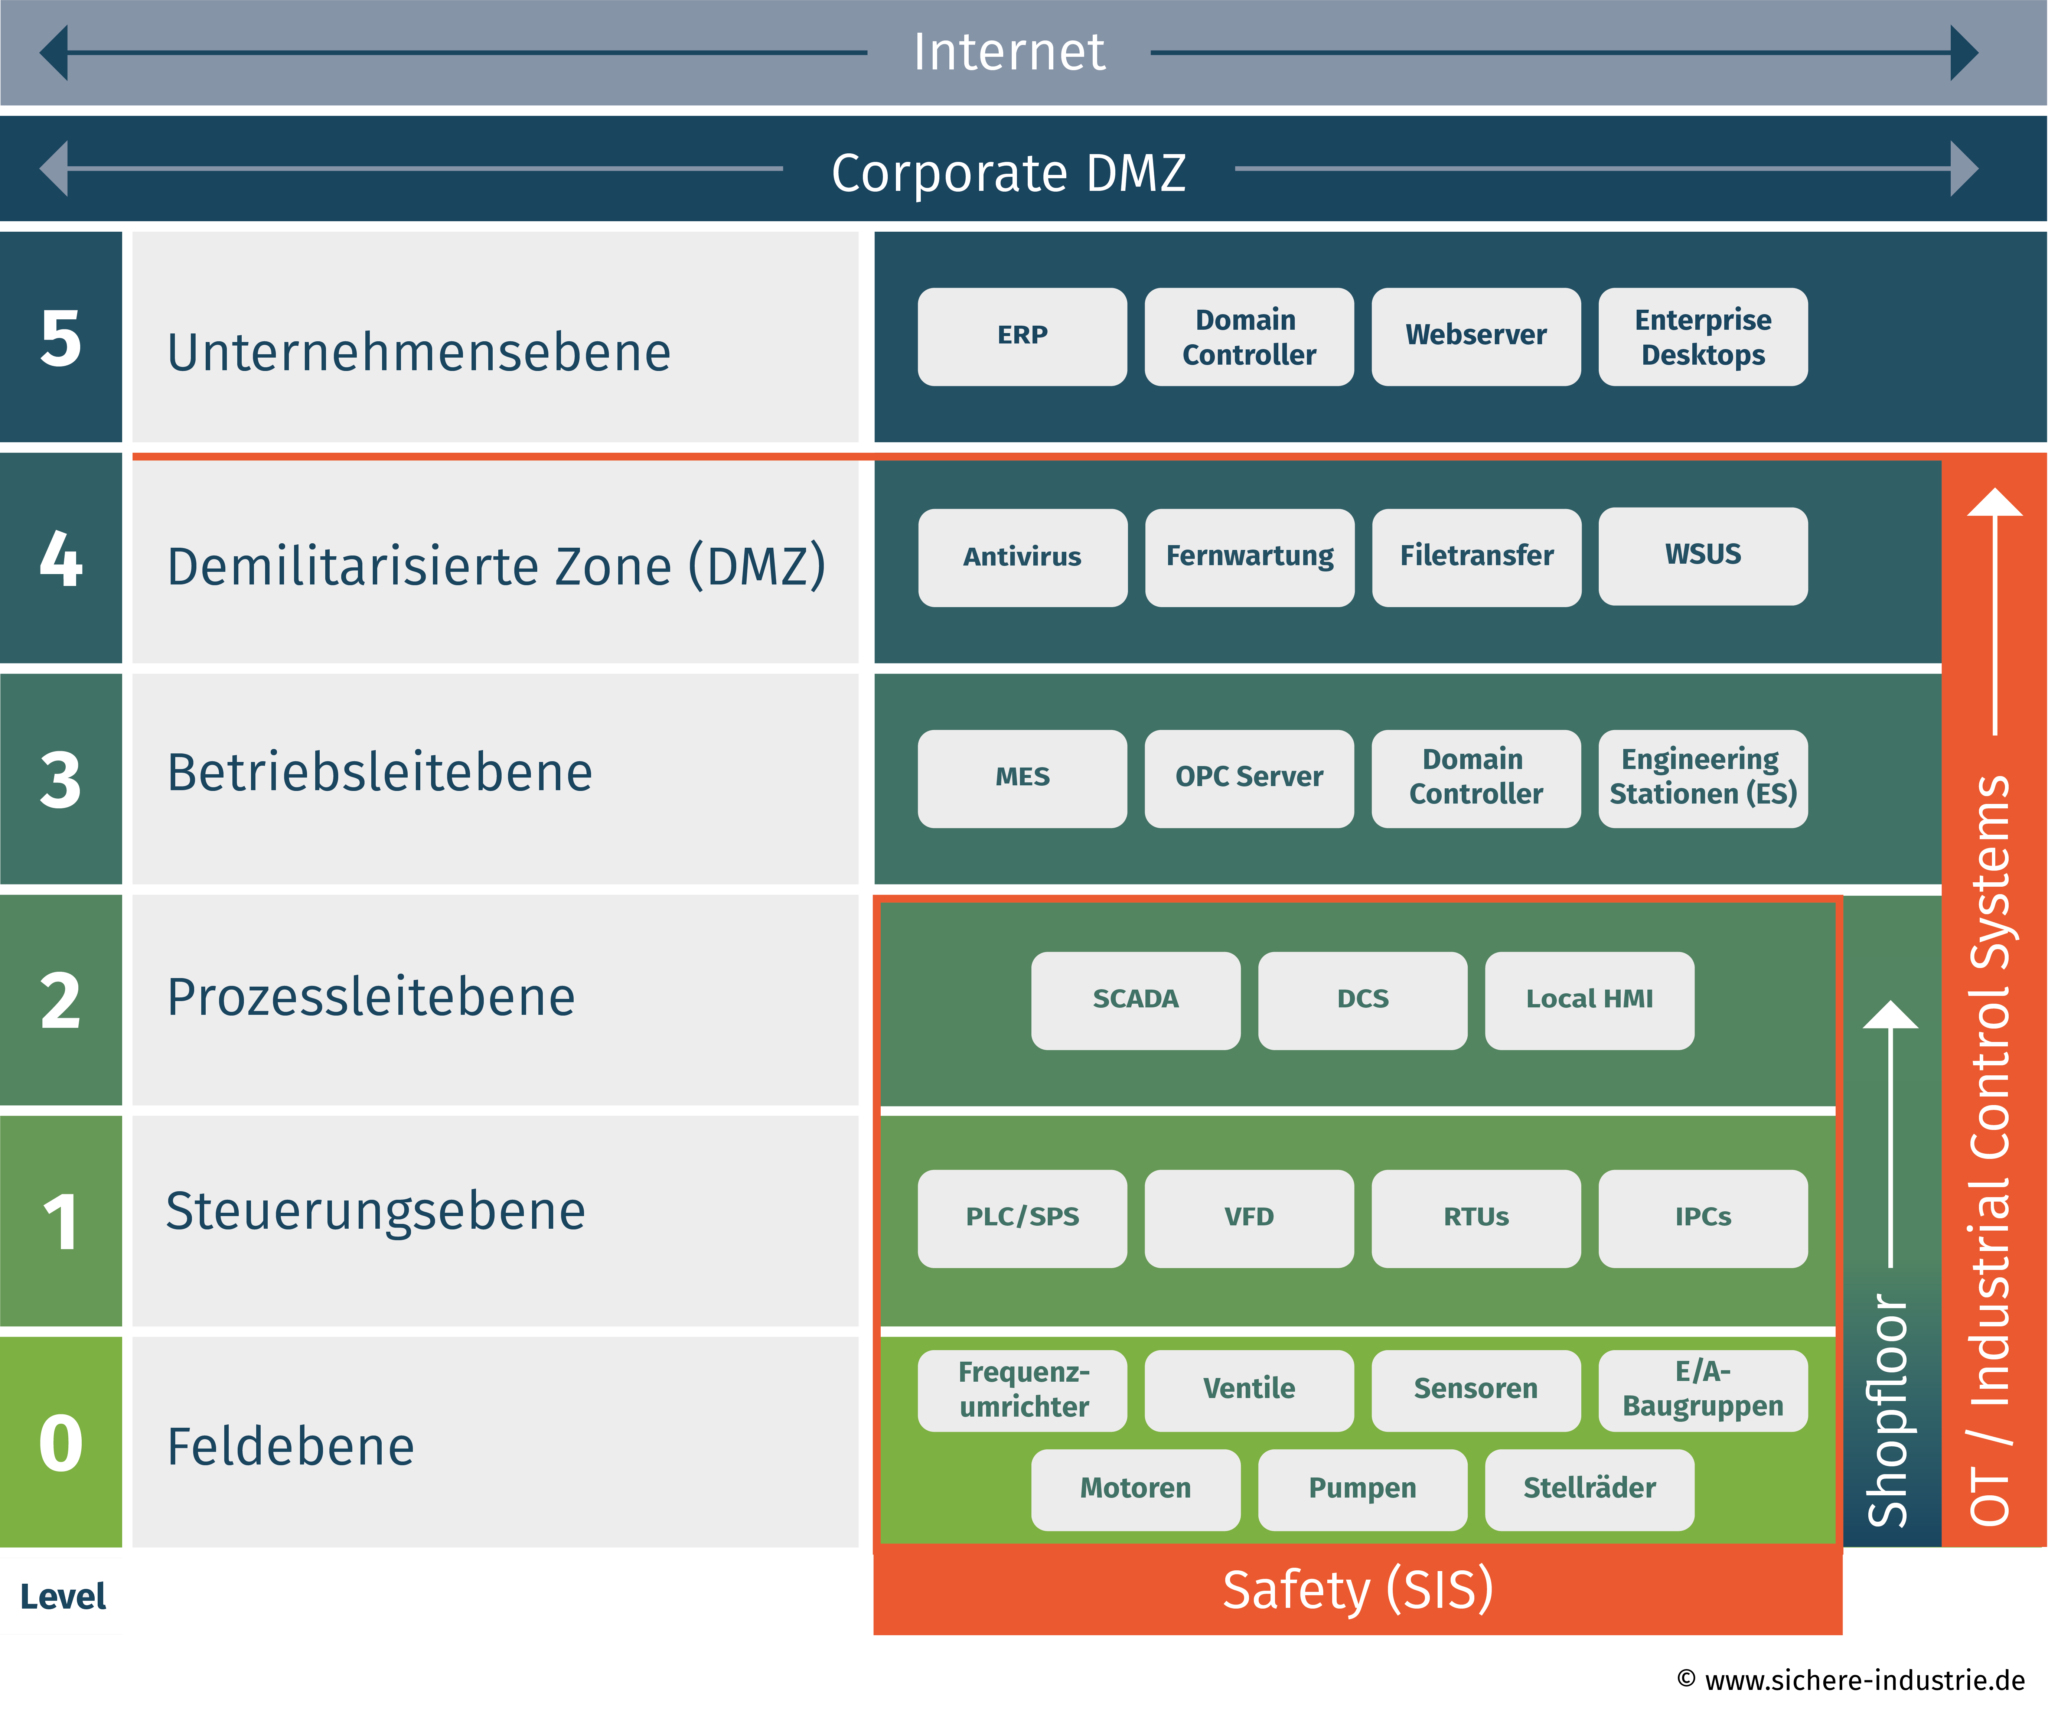
\includegraphics[width=0.8\textwidth]{images/Purdue_Modell.png} % Das Bild nimmt jetzt nur 50% der Textbreite ein
    \caption{Purdue-Referenzmodell}
    \label{fig:purdue_modell}
    \vspace{0.5em} % Etwas Platz zwischen der Bildunterschrift und der Quelle
    \centering
    \textit{Quelle: https://www.sichere-industrie.de/purdue-model/ (Besucht am 02.09.2024)} % Quelle zentriert
\end{figure}


\noindent Auf der höchsten Ebene, dem Unternehmensnetzwerk (Level 5), werden administrative Funktionen wie Buchhaltung, Vertrieb und Personalwesen unterstützt. Dieses Netzwerk bildet die Schnittstelle zu den operativen Anlagennetzen (Level 3) und gilt als besonders anfällig für Sicherheitsrisiken. Typische Systeme hier sind ERP-Systeme, Internetzugang, Fernwartungszugänge und Büroarbeitsplätze. Level 4, die \ac{dmz}, dient als Puffer zwischen höher geschützten Bereichen und dem Internet. Sie wird traditionell zwischen Office-Netzwerk und Internet platziert, um Systeme wie Webserver zu schützen. In einem industriellen Kontext trennt die DMZ den Office-Bereich vom Anlagennetzwerk und ermöglicht die Integration gemeinsamer Ressourcen wie Antivirus-Systemen und Fernwartungssystemen. Auf Level 3, der Betriebsleitebene, sind Systeme integriert, die für die Verwaltung und Überwachung der Produktionsabläufe verantwortlich sind. Dazu gehören Anlagen-IT-Komponenten, Engineering-Stationen und Manufacturing Execution Systems, die alle notwendigen Ressourcen für das Industrienetzwerk bereitstellen. In Level 2, der Prozessleitebene, werden Systeme zur Überwachung und Steuerung von Prozessabläufen eingesetzt. Diese Systeme arbeiten nicht in Echtzeit, wodurch Störungen keine sofortige Auswirkung auf die Automationslösungen haben. \clearpage \noindent Typische Systeme sind HMI, Alarm- und Benachrichtigungssysteme sowie Prozessdatenspeicher. Level 1, die Prozesssteuerungsebene, umfasst Systeme, die direkt die physischen Prozesse überwachen und steuern. Diese Systeme, darunter SPS, SCADA, DCS und RTUs, arbeiten in Echtzeit, was bedeutet, dass Störungen sofort den automatisierten Prozess beeinflussen können. Auf der niedrigsten Ebene, Level 0, wird der physische Geschäftsprozess ausgeführt. Die Befehle der Systeme auf Level 1 werden hier in Echtzeit umgesetzt. Typische Systeme auf dieser Ebene sind Motoren, Ventile, Pumpen und Remote I/O. Dieses Modell zeigt, dass die Anforderungen an Verfügbarkeit und Echtzeitfähigkeit mit abnehmender Ebene steigen. Systeme auf niedrigeren Ebenen sind nicht darauf angewiesen, den Sicherheitsstandards höherer Ebenen zu vertrauen (vgl. \cite{sichereIndustrie2}). Letztlich stellt sich die Frage, ob ein Modell, dass in den 1990er Jahren entwickelt wurde immernoch zeitgemäß ist. Das Purdue-Modell hat sich als Standard für die Architektur industrieller Steuerungssysteme etabliert, indem es klare Hierarchien zur Verbesserung der Kommunikationssicherheit schafft. Diese Struktur definiert, wie Maschinen und Prozesse zusammenarbeiten sollen. Mit dem Fortschritt im Industrial Internet of Things und der Integration smarter Funktionen in Sensoren und Steuerungen wird die traditionelle hierarchische Datenflussstruktur des Purdue-Modells zunehmend hinterfragt. In modernen Steuerungsarchitekturen ist es nicht mehr erforderlich, Daten durch alle Ebenen des Purdue-Modells zu leiten. Sensorendaten können direkt zur Cloud übermittelt werden, was neue Nutzungsmöglichkeiten eröffnet. Dennoch bleibt das Purdue-Modell wichtig für die Segmentierung von Netzwerken und den Schutz des OT-Netzes vor Sicherheitsbedrohungen. Daher ist es sinnvoll, eine hybride Lösung zu entwickeln, die die Prinzipien des Purdue-Modells bewahrt, aber gleichzeitig die Flexibilität für IIoT-Anwendungen bietet. Dies gewährleistet sowohl die Sicherheit als auch die Anpassungsfähigkeit (vgl. \cite{securityInsider}).



\subsection{Regulierungen und Standards}
Standards und Richtlinien spielen in der OT eine zentrale Rolle, indem sie Organisationen Leitlinien für den Schutz ihrer OT-Infrastrukturen bieten. Die internationale Normenreihe IEC 62443 behandelt umfassend die Cybersecurity für \ac{iacs} und verfolgt einen integrativen Ansatz für Betreiber, Integratoren und Hersteller im Bereich der Industrieautomatisierung. Somit setzt sie auf bereits etablierte Standards der ISO 27001 auf, welche auch Leitlinien für den Einsatz in der OT-Security gibt. Da diese sich tendenziell jedoch mit klassischen IT-Systemen auseinandersetzt, wird diese im folgenden nicht tiefgreifender erläutert. Die Entwicklung der IEC 62443 begann vor etwa 20 Jahren und wurde von der International Society for Automation (ISA) initiiert. \clearpage \noindent Diese Normenreihe legt detaillierte Verfahren zur sicheren Implementierung und Verwaltung von IACS fest und umfasst alle Industriebereiche sowie KRITIS. Ursprünglich aus der Automatisierungstechnik der Prozessindustrie hervorgegangen, hat sich die IEC 62443 auf sämtliche Industriebereiche ausgeweitet. Der Begriff IACS bezieht sich auf alle Komponenten, sowohl Hardware als auch Software, sowie auf die organisatorischen Prozesse, die für den zuverlässigen und sicheren Betrieb automatisierter Produktionsanlagen erforderlich sind. Die Norm zielt darauf ab, Normen, Verfahren und technische Berichte bereitzustellen, die Sicherheitsprozesse für die Implementierung von IACS definieren (\cite{DKE}). Betreiber, Hersteller und Integratoren von IACS und KRITIS sollen durch die Norm befähigt werden, Sicherheitsanfälligkeiten in ihren Systemen und Produkten zu identifizieren und zu beheben. Hierbei werden sowohl technische Aspekte der Hard- und Softwarekomponenten als auch prozessuale Aspekte, wie etwa in der Produktentwicklung, berücksichtigt.
Die Normenreihe ist in vier Hauptabschnitte unterteilt. Der erste Abschnitt, „General“, behandelt allgemeine Konzepte, Methoden und grundlegende Begriffe. Der zweite Abschnitt, „Policies and Procedures“, enthält Leitlinien und Verfahrensweisen zum Management der industriellen OT-Sicherheit. Im dritten Abschnitt, „System“, werden Vorgaben für Sicherheitsfunktionen von industriellen Automatisierungssystemen definiert. Der vierte Abschnitt, „Components and Requirements“, beschreibt die Anforderungen an Entwicklungsprozesse für sichere IACS-Produkte und -Komponenten.
Zusätzlich beschreibt die Normenreihe verschiedene Reifegrade von Prozessen und definiert unterschiedliche Sicherheitslevel für technische Anforderungen. Der niedrigste Sicherheitslevel (Level 0) erfordert keine besonderen Schutzmaßnahmen, während der höchste Sicherheitslevel (Level 4) umfassenden Schutz gegen gezielte Angriffe und Missbrauch durch Angreifer mit fortschrittlichen Mitteln und umfangreichen Ressourcen bietet (\cite{ISecInsider}). Das "Defense-in-Depth"-Prinzip ist ein Grundsatz, der ursprünglich aus dem Militär stammt und sicherstellen soll, dass sich Störfälle nicht durch das Ausschalten einer einzelnen Schutzmaßnahme ungehindert ausbreiten können. Um ein Sicherheitskonzept umzusetzen, müssen die Sicherheitsvorkehrungen aller Systeme, Produkte oder auch Richtlinien optimiert werden. Daher ergeben sich verschiedene Schichten (Zwiebelmodell), sodass beim Umgehen einer Schicht stets der Schutz durch die darauf folgende Schicht gewährleistet ist. Die IEC 62443 führt auch die Security-Level und Maturity-Level ein. Anhand der Security-Level werden die Systeme nach dem Sicherheitsaspekt bewertet. Das Maturity-Level hingegen konzentriert sich auf die Einhaltung organisatorischer Richtlinien. (vgl. \cite{sichereIndustrie3}). Neben der IEC 62443, die sich auf die Sicherheit industrieller Automatisierungssysteme konzentriert, bietet die NIST Special Publication 800-82 einen weiteren wichtigen Rahmen für den Schutz der OT. Die NIST Special Publication 800-82 bietet detaillierte Leitlinien zur Sicherung von ICS, die in kritischen Infrastrukturen wie Energieversorgung und Fertigung eingesetzt werden. \clearpage \noindent Da ICS zunehmend vernetzt sind, steigt das Risiko von Cyberangriffen, die nicht nur digitale, sondern auch physische Schäden verursachen können. SP 800-82 adressiert diese Herausforderungen, indem sie Organisationen einen strukturierten Ansatz zur Risikobewertung und Implementierung von Sicherheitskontrollen bietet. Der Standard deckt wesentliche Aspekte wie Zugangskontrollen, Netzwerksicherheit und die Reaktion auf Sicherheitsvorfälle ab, wobei er die Notwendigkeit eines kontinuierlichen Betriebs und die Integration von Legacy-Systemen berücksichtigt. Durch praxisnahe Empfehlungen und Fallstudien unterstützt SP 800-82 Organisationen dabei, eine robuste Sicherheitsstrategie zu entwickeln, die den Schutz kritischer Infrastrukturen gewährleistet. Die Anwendung dieses Standards ist ein zentraler Schritt zur Reduzierung von Sicherheitsrisiken und zur Sicherstellung der Integrität und Verfügbarkeit in OT-Umgebungen (\cite{NIST}).

\subsection{Fallbeispiele}
\subsubsection{STUXNET}

Im Bereich der Cybersicherheit und kritischen Infrastrukturen markiert das Jahr 2010 einen bedeutenden Meilenstein durch das Auftreten des Stuxnet-Wurms. Diese hochentwickelte Schadsoftware wurde entdeckt, als sie erfolgreich Zugang zu einem wichtigen industriellen Steuerungssystem verschaffte, das Teil eines Urananreicherungsprogramms im Iran war (vgl. \cite{Stuxnet}, S. 1 ff.). Die Auswirkungen waren drastisch: Etwa 1000 Uranzentrifugen wurden schwer beschädigt, was eine umfangreiche und kostspielige Reparatur erforderlich machte. Neu daran war, dass Cyberattacken zuvor nur indirekt die Grenze zur physikalischen Welt überschritten hatten. Dies änderte sich mit Stuxnet, da industrielle Anlagen direkt gestoppt und zerstört wurden (vgl. \cite{Fraunhofer}, S. 12). Stuxnet war bahnbrechend, weil es als erste Schadsoftware bekannt wurde, die über USB-Laufwerke Zielgeräte infizierte. Darüber hinaus konnte sich der Wurm eigenständig aktualisieren, indem er Peer-to-Peer-Kommunikation\footnote{Teilnehmer direkt miteinander verknüpft mit gleichen Rechten} und Online-Verbindungen nutzte. Durch den Einsatz einer gestohlenen digitalen Signatur gelang es ihm, ein Rootkit\footnote{Softwarewerkzeuge, die ermöglichen zukünftige Anmeldevorgänge des Eindringlings zu verbergen sowie Prozesse und Dateien zu tarnen} zu installieren, was seine fortschrittlichen und zielgerichteten Angriffsmethoden verdeutlichte (vgl. \cite{NordVPN}).
\clearpage
\subsubsection{TRISIS}

Der Vorfall mit TRISIS\footnote{auch häufig unter TRITON bekannt} im Sommer 2017 markierte einen bedeutenden Zwischenfall im Bereich der kritischen Infrastrukturen, insbesondere in einem Chemiewerk in Saudi-Arabien. Ursprünglich als technischer Fehler in den Safety-Systemen des Herstellers Schneider Electric vermutet, stellten Sicherheitsexperten fest, dass dieser Vorfall auf eine gezielte Schadsoftware zurückzuführen war. Die Malware, bekannt als TRISIS, sollte die TRICONEX Safety-Systeme, die für sicherheitsrelevante Aktionen in der Anlage zuständig sind infiltrieren und hatte potenziell katastrophale Auswirkungen, wäre der Fehler nicht entdeckt worden. Dieser Befall wurde günstigerweise durch einen Fehler im Code der Schadsoftware gefunden. Der Angriff nutzte mehrere Schwachstellen aus, darunter einen offen zugänglichen Schlüsselschalter im Programmiermodus sowie unzureichende Netzwerksegmentierung, die den Angreifer Zugang zur Engineering-Station verschafft hätten. Diese Station wurde verwendet, um das Safety-System zu programmieren, und bot damit eine Eintrittspforte für die Schadsoftware. TRISIS wurde speziell für TRICONEX-Systeme entwickelt und zielte darauf ab, sicherheitsrelevante Prozesse zu manipulieren oder zu stören. Der Vorfall weist auf die Gefahr hin, dass auch hochsichere Systeme anfällig für digitale Angriffe sind, unabhängig von der Qualität oder Herkunft der verwendeten Software. TRISIS wird häufig mit der Hackergruppe APT33 in Verbindung gebracht, die mit dem iranischen Staat assoziiert wird. Jedoch ist eine konkrete Zuordnung von Cyberattacken zu bestimmten staatlichen Institutionen selten eindeutig vornehmbar. Während keine unmittelbaren physischen Schäden gemeldet wurden, verdeutlicht dieser Vorfall die potenziellen Risiken staatlich finanzierter Cyberangriffe, die gezielt industrielle Steuerungssysteme ins Visier nehmen. Die komplexe Natur von TRISIS und seine spezifische Ausrichtung legen nahe, dass der Angriff möglicherweise für einen begrenzten Kreis entwickelt wurde, jedoch schwerwiegende Konsequenzen gehabt hätte, wenn er erfolgreich gewesen wäre. Für zukünftige Sicherheitsmaßnahmen wird empfohlen, Safety-Systeme strikt vom restlichen Automatisierungsnetzwerk abzuschotten oder sogar physisch zu isolieren (vgl. \cite{TRISIS}).

\subsubsection{Industroyer}

Industroyer ist eine spezialisierte Malware, die 2016 erstmals entdeckt wurde und gezielt industrielle Steuerungssysteme angreift. Der Angriff führte zu einem großflächigen Stromausfall in Kiew, Ukraine. Am 17. Dezember 2016 kam es in Kiew zu schweren Stromausfällen aufgrund des unerwarteten Abschaltens mehrerer Umspannwerke. Das slowakische IT-Sicherheitsunternehmen ESET untersuchte daraufhin die Netzleitsysteme und identifizierte eine komplexe Schadsoftware, die unter dem Namen Win32/Industroyer bekannt wurde.\clearpage \noindent Eine weitergehende Analyse durch das US-amerikanische Unternehmen Dragon Inc. ergab, dass die Malware sich selbst als ,,CRASH`` identifizierte, woraufhin sie auch als Crashoverride bekannt wurde. Die Analysen beider Unternehmen bestätigten, dass Industroyer eine hochentwickelte Malware ist, die speziell für die Beeinflussung physischer Komponenten in industriellen Steuerungssystemen entwickelt wurde (vgl. \cite{rhebo}). Die Bedrohung durch Industroyer ergibt sich insbesondere aus der Fähigkeit, industrielle Kommunikationsprotokolle auf eine Art und Weise zu nutzen, die diesen ursprünglich vorgesehen war. Diese Protokolle, die vor Jahrzehnten entwickelt wurden, waren damals nicht auf Sicherheitsaspekte ausgerichtet, da die industriellen Systeme primär in isolierten Umgebungen betrieben wurden. In der heutigen Zeit, in der industrielle Systeme zunehmend mit externen Netzwerken verbunden sind, zeigen sich Schwächen, die durch diese veralteten Protokolle nicht adressiert wurden. Cyber-Kriminelle benötigen daher keine tiefgehende Analyse von Schwachstellen innerhalb der Protokolle selbst. Stattdessen reicht es aus, dass sie ihre Schadsoftware mit der Fähigkeit ausstatten, die bestehenden Protokollsprachen zu verstehen und anzuwenden. Diese Vorgehensweise ermöglicht es Angreifern, bestehende Kommunikationskanäle gezielt auszunutzen und industrielle Systeme zu manipulieren, ohne dass zusätzliche Sicherheitsmechanismen implementiert wurden (vgl. \cite{welivesecurity}). 

\subsection{Zukunft der OT-Security}

Angesichts der dynamischen Bedrohungslandschaft ist es essenziell, zukünftige Entwicklungen und innovative Sicherheitslösungen zu erforschen, um die Resilienz gegenüber neuen Risiken und Herausforderungen zu stärken. Der Einsatz von \ac{ki} gewinnt zunehmend an Bedeutung in der Sicherheitsbranche, da er sowohl neue Angriffsmöglichkeiten eröffnet als auch fortschrittliche Abwehrstrategien ermöglicht. KI-Technologien bieten den entscheidenden Vorteil, dass sie Bedrohungen und Anomalien erheblich schneller und präziser erkennen können als Menschen. Diese Systeme entwickeln sich kontinuierlich weiter und passen sich dynamisch an neue Gefahren an, was in einer sich ständig verändernden Sicherheitslandschaft unverzichtbar ist. Durch Anomalieerkennung, Verhaltensanalyse und prädiktive Methoden kann KI potenzielle Gefahren frühzeitig identifizieren, indem sie ungewöhnliche Muster und Verhaltensweisen im System aufspürt (vgl. \cite{hornetsec}). Besonders hervorzuheben ist die Fähigkeit von KI-Systemen, Bedrohungen in Echtzeit zu erkennen und sofortige Warnungen auszugeben, was eine schnelle Reaktion ermöglicht. Darüber hinaus können diese Systeme autonom Schutzmaßnahmen ergreifen, was besonders außerhalb der üblichen Arbeitszeiten von großer Bedeutung ist. Allerdings bringt der Einsatz von KI auch spezifische Herausforderungen mit sich.\clearpage \noindent Die Integration in bestehende Systeme kann komplex und technisch anspruchsvoll sein, was organisatorische Hürden aufwirft. Zudem benötigen KI-Systeme große Mengen an qualitativ hochwertigen Daten, um zuverlässig arbeiten zu können. Die Komplexität dieser Systeme kann zudem die Effizienz bei der Fehlersuche und Weiterentwicklung beeinträchtigen (vgl. \cite{itPort}). Das Zero-Trust-Modell wird zunehmend an Bedeutung gewinnen. Dieses benennt kein implizites Vertrauen, da jeder Datenaustausch erst nach strenger Authentifizierung und Autorisierung erfolgt. Viele Normierungen sind ausschließlich auf IT ausgelegt. Daher ist zu erwarten, dass strengere regulatorische Anforderungen und Normen zur OT-Security erlassen werden. Diese werden Unternehmen dazu zwingen, ihre Sicherheitspraktiken zu verbessern und regelmäßig Audits durchzuführen. Neue Technologien wie Edge-Computing können auch immer wichtigere Rollen im Bereich der OT-Security erlangen. Dabei handelt es sich um eine Methode der Datenverarbeitung, bei der die Verarbeitung direkt oder in unmittelbarer Nähe zur Datenquelle erfolgt. Dies reduziert die Notwendigkeit, Daten an entfernte Rechenzentren zu senden und dort zu verarbeiten. Edge Computing erleichtert die Integration von IT- und OT-Netzwerken, indem es eine Plattform bietet, die Daten fast in Echtzeit verarbeitet und so das nahtlose Teilen wichtiger Daten ermöglicht. Dies fördert die Zusammenarbeit der beiden Teams, indem sie ihre Ressourcen und Fachkenntnisse bündeln (vgl. \cite{stratus}). Es ist abzusehen, dass Angriffe auf OT in Zukunft vermehrt stattfinden werden. Angreifer entwickeln immer fortschrittlichere Angriffsmethoden um in Netzwerke einzudringen. Unter anderem werden auch die Angriffsflächen größer, da ICS immer vernetzter werden und OT-Geräte so über Netzwerke zugänglich sind, was von Angreifern ausgenutzt werden kann. Diese Systeme laufen häufig mit veralteten Betriebssystem und Software, da das Patchen mit Risiken und Kosten verbunden ist, welche oft weniger gute Abwehrmechanismen vor Cyberangriffen haben. 

